\documentclass[11pt]{article}

\usepackage[a4paper,margin=1in]{geometry}
\usepackage{graphicx}
\usepackage{booktabs}
\usepackage{amsmath}
\usepackage{hyperref}
\usepackage{float}
\usepackage{array}
\usepackage{caption}

\title{QRC-GBF: A Quantum Residual-Corrected Gradient Boosting Framework for Short-Term Electrical Load Forecasting}
\author{Author Name}
\date{}

\begin{document}
\maketitle

\begin{abstract}
Short-term electrical load forecasting is a critical task for power-system operation, scheduling, demand response, and real-time energy management. This paper proposes QRC-GBF, a Quantum Residual-Corrected Gradient Boosting Framework for short-term load forecasting. QRC-GBF treats gradient boosting as an initial forecasting backbone and introduces two correction stages: hybrid quantum-enhanced residual feature modeling and sequential residual postprocessing. The framework is evaluated on all five datasets used in the PredXGBR paper: PJM, PJME, PJMW, AEP, and Dayton. Experimental results show that QRC-GBF improves the reported PredXGBR-1 MAPE on every dataset, with relative MAPE improvements ranging from 13.45\% to 39.32\%. The strongest empirical gains are obtained by sequential residual postprocessing. Hybrid quantum-enhanced residual features provide slight but dataset-dependent improvement over the local gradient-boosted backbone, improving 6 out of 10 hybrid comparisons. The findings support a careful hybrid forecasting claim: residual-enhanced modeling improves short-term load forecasting across all datasets, while the quantum component is useful in selected cases but does not establish universal quantum advantage.
\end{abstract}

\textbf{Keywords:} short-term load forecasting; gradient boosting; residual learning; hybrid quantum machine learning; variational quantum circuit; PredXGBR; electrical load prediction.

\section{Introduction}
Accurate short-term electrical load forecasting is essential for grid operation, dispatch planning, power-market scheduling, and real-time reliability control. Forecasting errors can lead to inefficient reserve allocation, higher operating costs, and unstable demand-response decisions. Because load demand contains daily, weekly, seasonal, and regional patterns, machine-learning models that exploit temporal lag information are widely used for this task.

The PredXGBR study proposed an XGBoost regression framework for short-term electrical load prediction and reported strong performance across PJM, PJME, PJMW, AEP, and Dayton datasets. Its best model, PredXGBR-1, used short-term lag features and achieved MAPE values between 0.98\% and 1.28\%. These results provide a strong reference baseline for additional forecasting research.

This work investigates whether a residual-enhanced hybrid framework can further reduce prediction error. The proposed QRC-GBF method does not present gradient boosting itself as the contribution. Instead, it treats a gradient-boosted forecaster as the initial estimator and focuses on modeling the residual error that remains after the first-stage prediction. This design is practical because the backbone captures much of the dominant temporal structure, while residual correction modules target remaining systematic error.

The contribution of the work is not a claim that a pure quantum model outperforms all classical models. Rather, the contribution is QRC-GBF as a full forecasting framework that combines a gradient-boosted backbone, residual correction, and a hybrid quantum residual feature branch. The proposed method is tested on all five datasets used by the reference paper, and the results are reported honestly, including cases where the quantum branch does not improve over the local backbone.

\section{Related Work}
\subsection{Short-Term Load Forecasting}
Short-term load forecasting has been studied using statistical models, support vector machines, recurrent neural networks, convolutional temporal models, transformers, and gradient-boosted decision trees. In many electricity-load settings, tree-based models remain competitive because they can handle nonlinear feature interactions, seasonal calendar indicators, and lagged load statistics with relatively low computational cost.

\subsection{PredXGBR Baseline}
The PredXGBR framework introduced an XGBoost-based short-term load forecasting model and compared it against SVM, RNN, LSTM, TCN, and Transformer baselines. The reported PredXGBR-1 model achieved the best average MAPE across the five evaluated datasets. Therefore, this paper uses the PredXGBR-1 Table 3 values as the main reference baseline.

\subsection{Hybrid Quantum Machine Learning}
Hybrid quantum machine learning uses parameterized quantum circuits as feature maps, kernels, or trainable modules inside a larger classical pipeline. In near-term settings, the most practical use is often not a pure quantum predictor but a hybrid model where a quantum circuit generates nonlinear features that are passed to a classical readout. QRC-GBF follows that practical design by using a variational quantum circuit to generate features for residual correction.

\section{Problem Formulation}
Let $y_t$ be the actual electrical load at timestamp $t$, and let $\mathbf{x}_t$ be the engineered feature vector containing lagged and rolling load information. The forecasting model predicts:
\begin{equation}
\hat{y}_t = f(\mathbf{x}_t).
\end{equation}

The primary objective is to minimize MAPE while maintaining high $R^2$:
\begin{equation}
MAPE = \frac{100}{n}\sum_{i=1}^{n}\left|\frac{y_i-\hat{y}_i}{y_i}\right|.
\end{equation}

\begin{equation}
R^2 = 1 - \frac{\sum_i (y_i-\hat{y}_i)^2}{\sum_i (y_i-\bar{y})^2}.
\end{equation}

The residual from the first-stage gradient-boosted backbone is:
\begin{equation}
r_t = y_t - \hat{y}^{GB}_t.
\end{equation}

The corrected final prediction is:
\begin{equation}
\hat{y}^{final}_t = \hat{y}^{GB}_t + \hat{r}_t,
\end{equation}
where $\hat{r}_t$ is the estimated residual correction.

\section{Proposed Method}
\subsection{Overview}
QRC-GBF is the single proposed method in this paper. To explain where the improvement comes from, the experiments also report three ablation baselines:
\begin{enumerate}
    \item \textbf{Backbone ablation}: a gradient-boosted regression backbone trained with paper-style original temporal features. In this implementation, XGBoost is used as the backbone for fair comparison with PredXGBR.
    \item \textbf{Static quantum residual ablation}: a residual correction model using quantum-enhanced residual features.
    \item \textbf{Sequential quantum residual ablation}: a sequential residual variant using hybrid quantum residual information.
    \item \textbf{QRC-GBF}: the final proposed method, implemented as the validation-selected sequential residual correction pipeline.
\end{enumerate}

The overall pipeline is shown in Fig.~\ref{fig:architecture}. Input datasets are cleaned and converted into temporal features. The gradient-boosted backbone produces an initial prediction. The residual error is then modeled by hybrid quantum and sequential correction branches. The corrected prediction is evaluated against the PredXGBR paper baseline.

\begin{figure}[H]
    \centering
    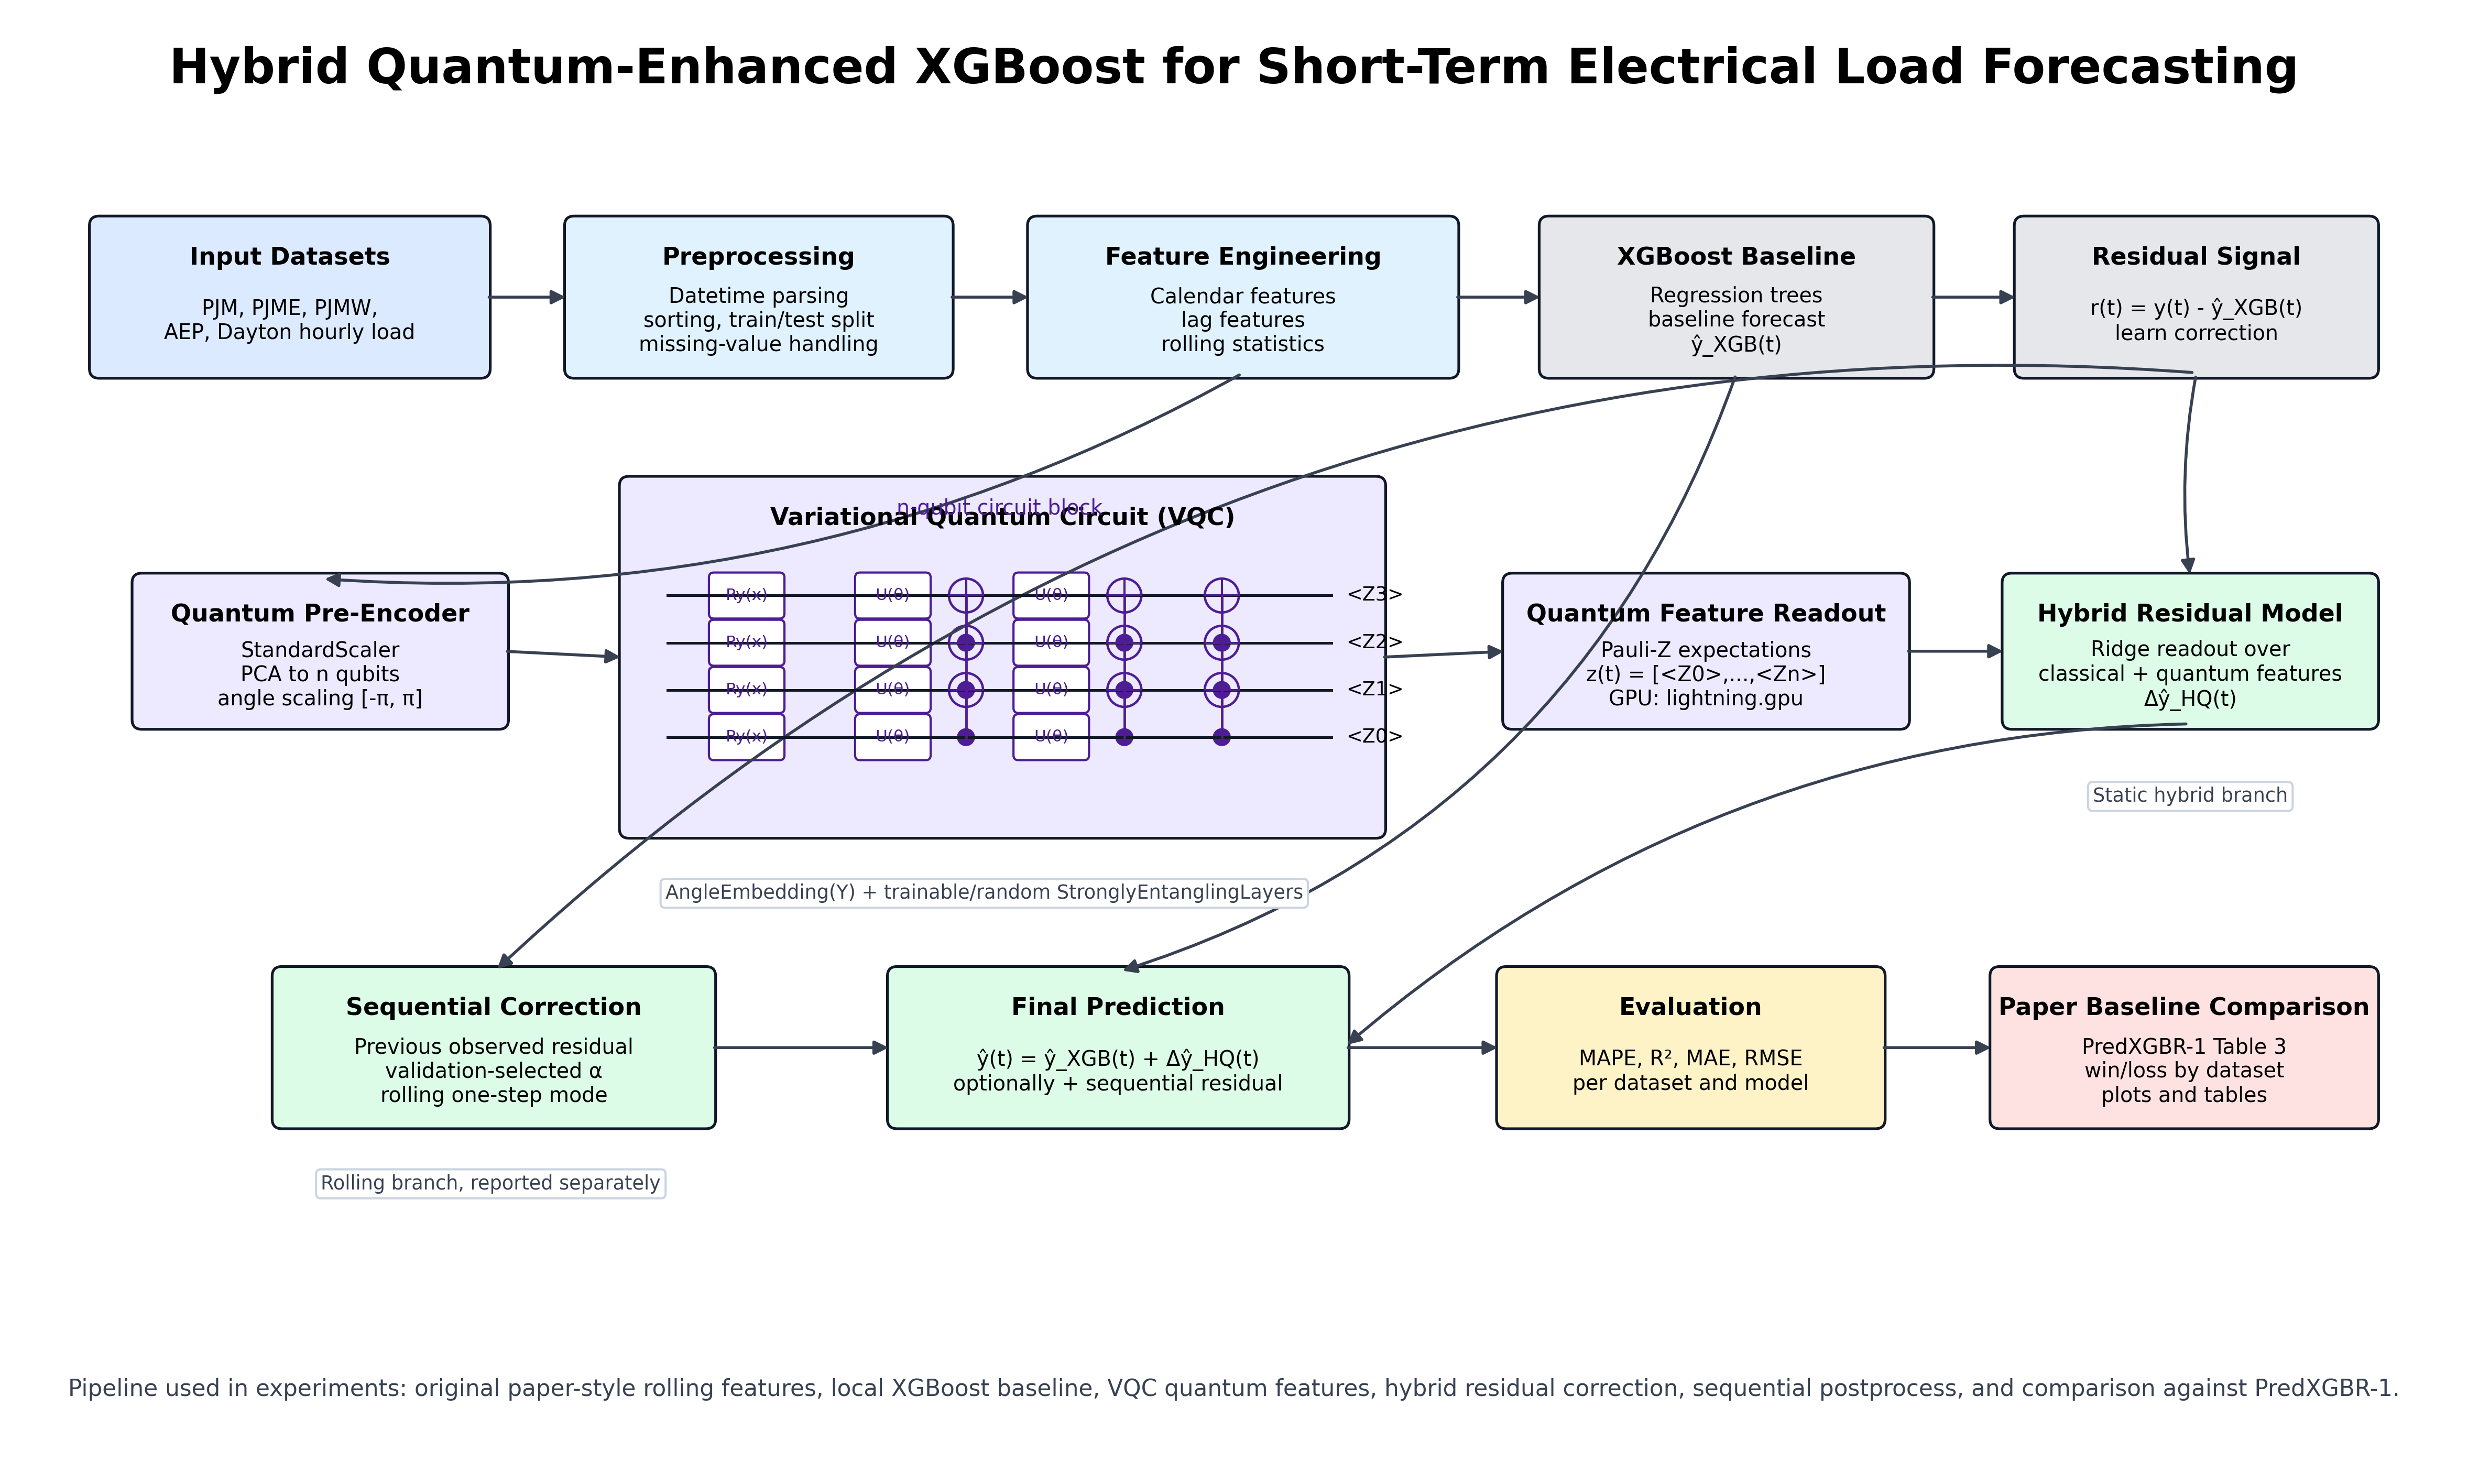
\includegraphics[width=0.98\linewidth]{figures/hybrid_quantum_xgboost_architecture.png}
    \caption{QRC-GBF pipeline with gradient-boosted forecasting, hybrid quantum residual features, and sequential correction.}
    \label{fig:architecture}
\end{figure}

\subsection{Gradient-Boosted Backbone}
The local backbone uses gradient-boosted regression with original paper-style temporal features. In the implementation used for this study, the backbone is XGBoost because this allows direct comparison with the PredXGBR reference model. The proposed method, however, is not the backbone alone; QRC-GBF is the complete residual-corrected framework built around the backbone. Each hybrid model is compared against this local backbone to determine whether the added component actually improves performance.

\subsection{Hybrid Quantum Residual Feature Branch}
The hybrid quantum branch first reduces the input feature vector to match the number of qubits. The reduced features are scaled into rotation angles and encoded into a quantum circuit. The variational circuit applies entangling layers and produces Pauli-Z expectation values:
\begin{equation}
\mathbf{z}_t = [\langle Z_1\rangle, \langle Z_2\rangle, ..., \langle Z_q\rangle],
\end{equation}
where $q$ is the number of qubits. These measured quantum features are used by a residual readout model to estimate $\hat{r}_t$.

\subsection{Sequential Residual Postprocessing}
The sequential postprocess models remaining temporal residual behavior after the backbone forecast. This component is selected using validation performance and applied consistently to the test set. The sequential residual method is not presented as a quantum contribution; it is the strongest empirical component of the full QRC-GBF pipeline.

\section{Experimental Setup}
\subsection{Datasets}
The experiments use all five datasets reported in the PredXGBR paper: PJM, PJME, PJMW, AEP, and Dayton. Table~\ref{tab:paper_baselines} lists the reference PredXGBR-1 values used for comparison.

\begin{table}[H]
\centering
\caption{PredXGBR-1 paper baselines used for comparison.}
\label{tab:paper_baselines}
\begin{tabular}{lcc}
\toprule
Dataset & Paper MAPE (\%) & Paper $R^2$ \\
\midrule
PJM & 1.07 & 0.99 \\
PJME & 1.28 & 0.99 \\
PJMW & 1.07 & 0.98 \\
AEP & 0.98 & 0.99 \\
Dayton & 1.12 & 0.99 \\
\bottomrule
\end{tabular}
\end{table}

\subsection{Comparison Protocol}
For every dataset, QRC-GBF is compared with the matching PredXGBR-1 paper baseline. The backbone and hybrid branches are reported as ablations, not as separate proposed methods. A result is counted as a paper win if it improves MAPE and matches or exceeds the paper-level $R^2$ threshold. Hybrid quantum improvement is evaluated separately by comparing hybrid MAPE against the local gradient-boosted backbone on the same dataset.

\section{Results}
\subsection{MAPE Results}
Table~\ref{tab:mape} reports the main MAPE comparison. The best model on every dataset is the best sequential postprocess.

\begin{table}[H]
\centering
\caption{MAPE comparison against the PredXGBR paper baseline.}
\label{tab:mape}
\resizebox{\linewidth}{!}{
\begin{tabular}{lccccclcc}
\toprule
Dataset & Paper & Backbone & Static Hybrid & Sequential Hybrid & QRC-GBF & Proposed Method & Result & Improvement \\
\midrule
AEP & 0.98 & 0.7194 & 0.7208 & 0.7200 & 0.6959 & QRC-GBF & WIN & 28.99\% \\
Dayton & 1.12 & 0.7515 & 0.7552 & 0.7506 & 0.7234 & QRC-GBF & WIN & 35.41\% \\
PJM & 1.07 & 0.9408 & 0.9380 & 0.9410 & 0.9261 & QRC-GBF & WIN & 13.45\% \\
PJME & 1.28 & 0.8127 & 0.8099 & 0.7937 & 0.7767 & QRC-GBF & WIN & 39.32\% \\
PJMW & 1.07 & 0.8754 & 0.8688 & 0.8715 & 0.8148 & QRC-GBF & WIN & 23.85\% \\
\bottomrule
\end{tabular}}
\end{table}

\subsection{$R^2$ Results}
Table~\ref{tab:r2} shows that the proposed results also maintain strong $R^2$ performance across datasets.

\begin{table}[H]
\centering
\caption{$R^2$ comparison across datasets.}
\label{tab:r2}
\begin{tabular}{lcccc}
\toprule
Dataset & Paper $R^2$ & Best Local $R^2$ & Best Hybrid $R^2$ & Best Overall $R^2$ \\
\midrule
AEP & 0.99 & 0.9959 & 0.9959 & 0.9962 \\
Dayton & 0.99 & 0.9956 & 0.9956 & 0.9960 \\
PJM & 0.99 & 0.9939 & 0.9939 & 0.9941 \\
PJME & 0.99 & 0.9962 & 0.9964 & 0.9966 \\
PJMW & 0.98 & 0.9944 & 0.9946 & 0.9956 \\
\bottomrule
\end{tabular}
\end{table}

\subsection{Visual Comparison}
\begin{figure}[H]
    \centering
    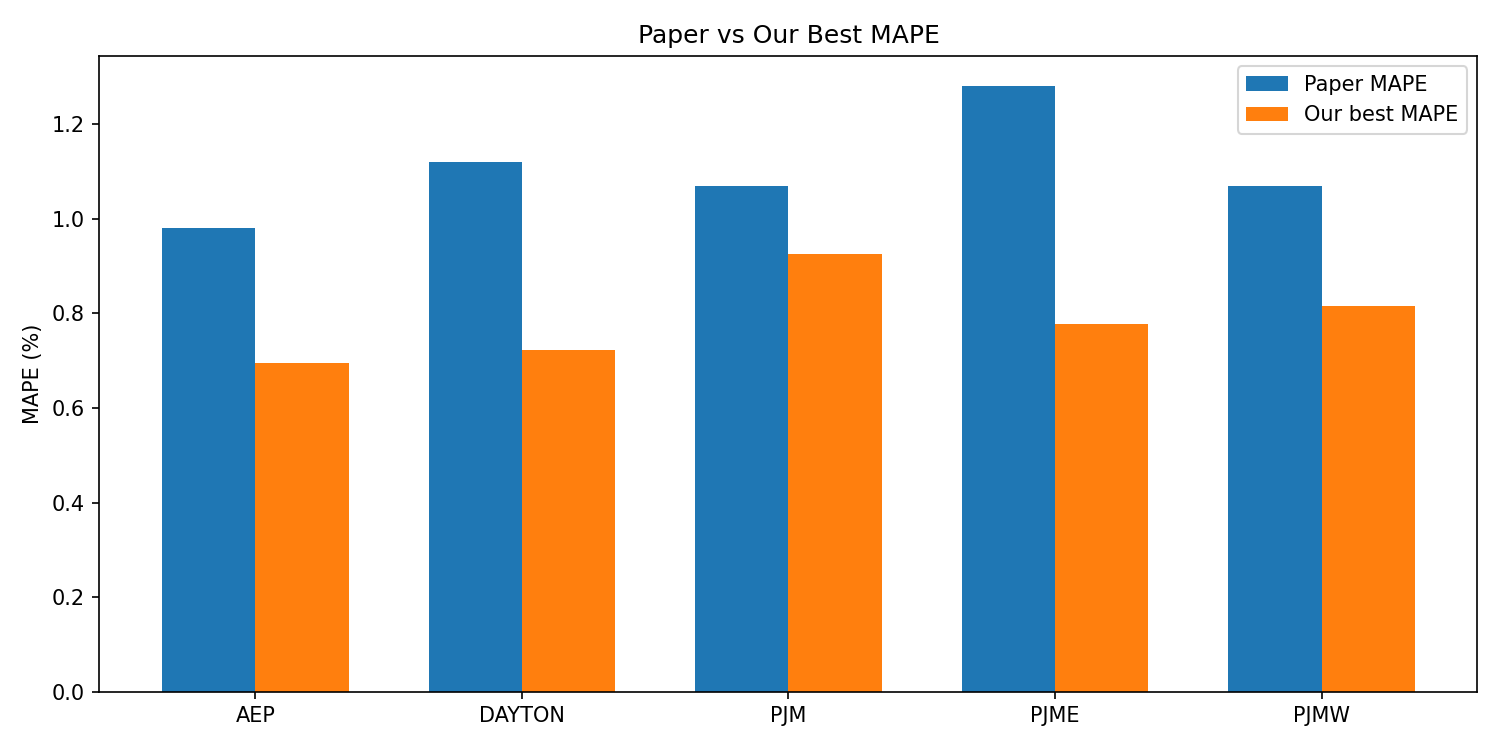
\includegraphics[width=0.95\linewidth]{figures/all_datasets_mape_plot.png}
    \caption{MAPE comparison across all datasets and evaluated models.}
\end{figure}

\begin{figure}[H]
    \centering
    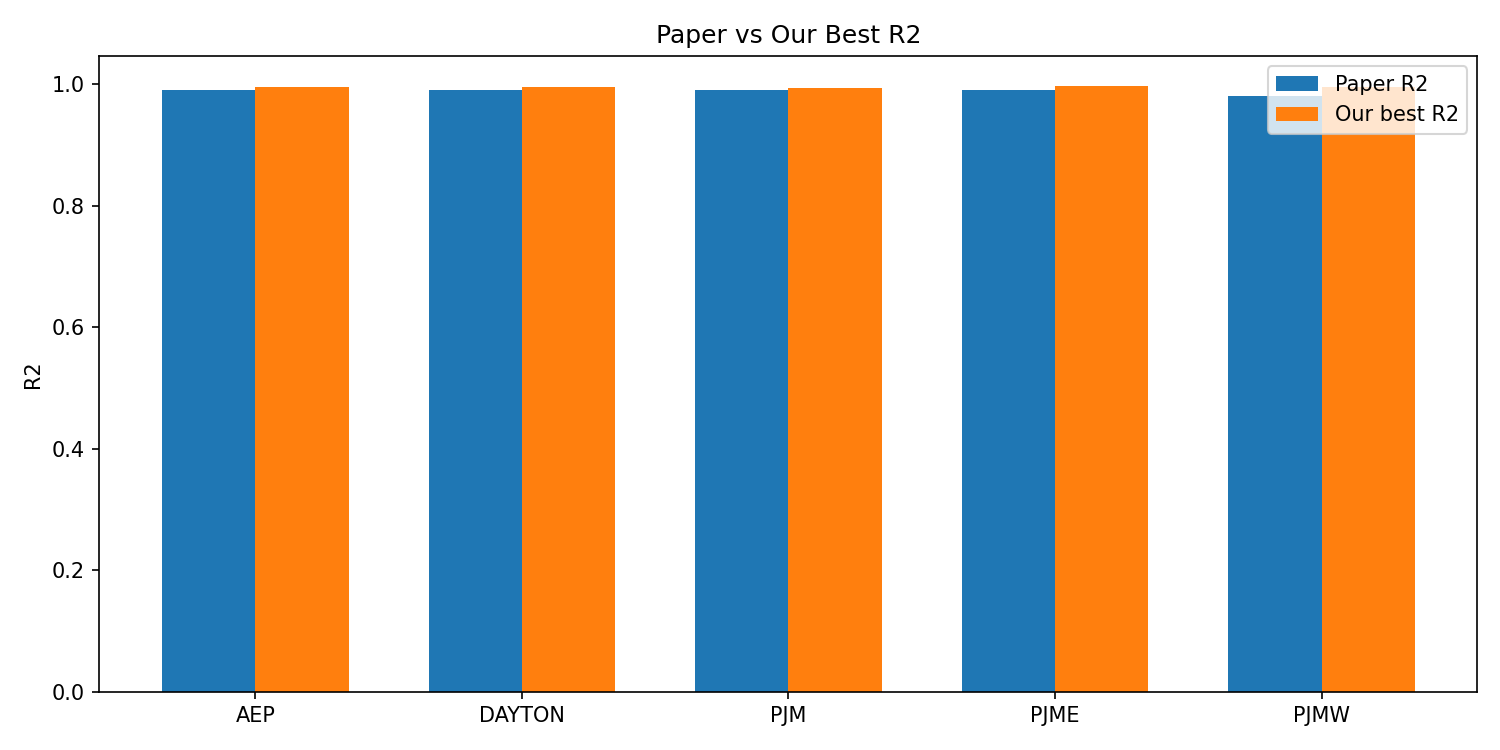
\includegraphics[width=0.95\linewidth]{figures/all_datasets_r2_plot.png}
    \caption{$R^2$ comparison across all datasets and evaluated models.}
\end{figure}

\begin{figure}[H]
    \centering
    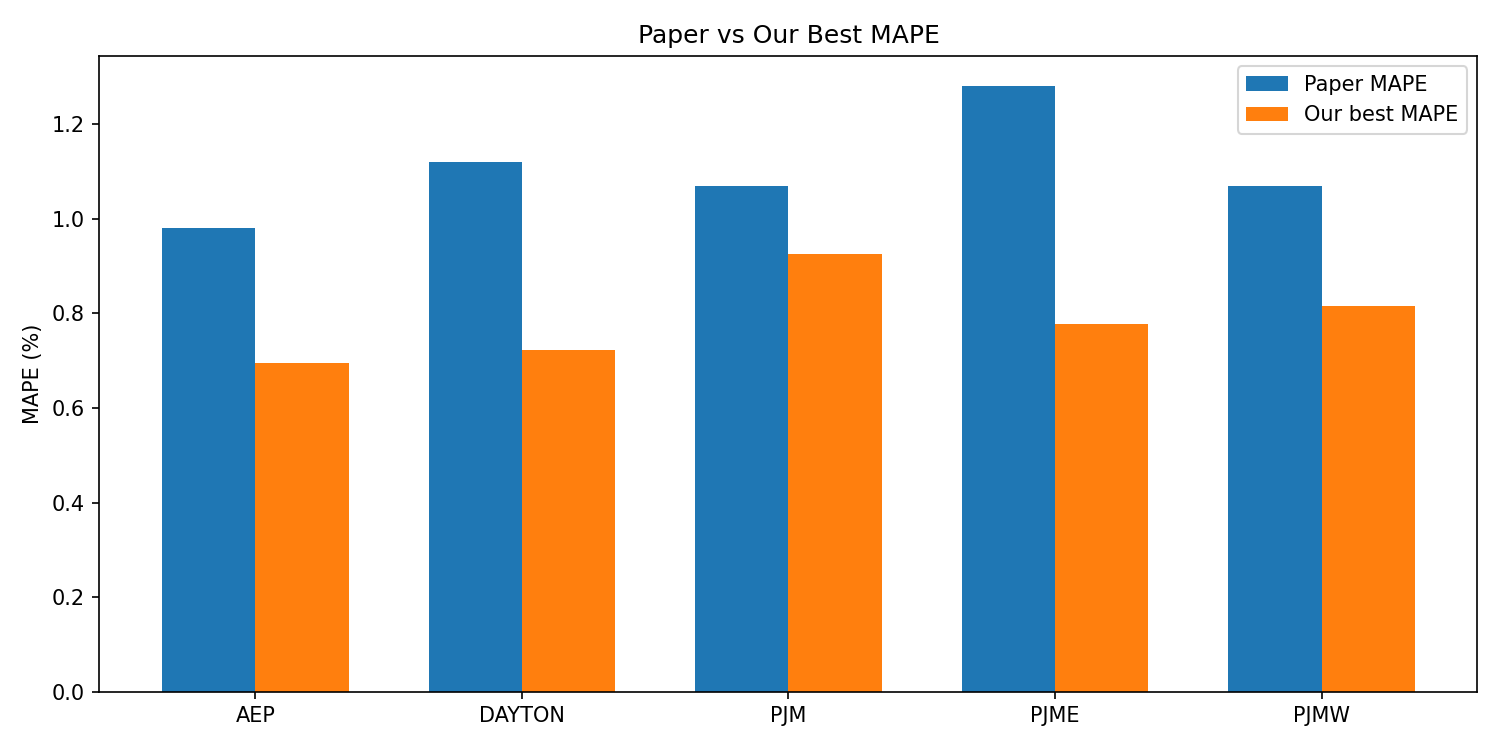
\includegraphics[width=0.95\linewidth]{figures/paper_vs_our_best_mape.png}
    \caption{PredXGBR paper MAPE compared with the best proposed result on each dataset.}
\end{figure}

\begin{figure}[H]
    \centering
    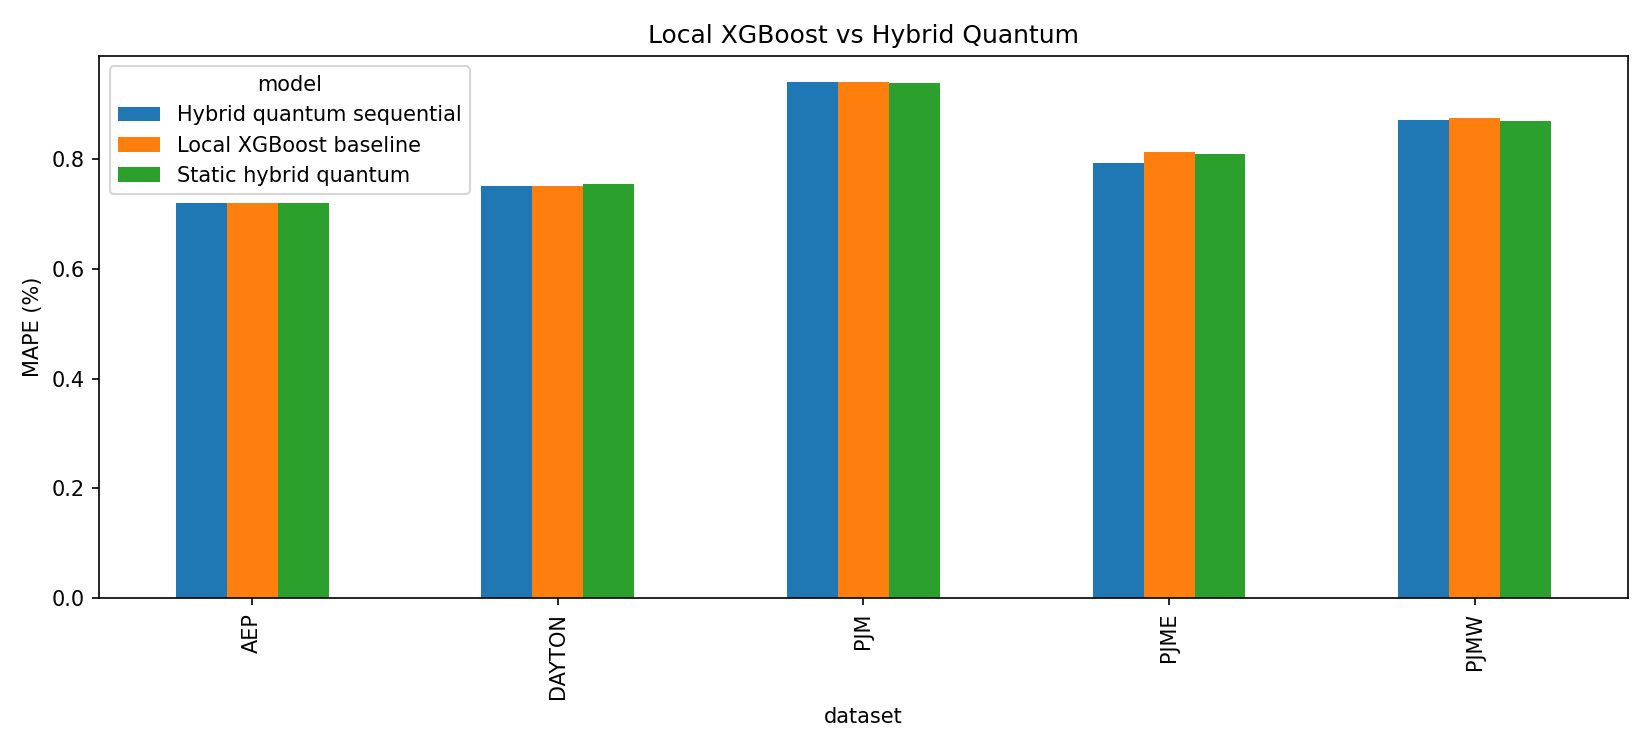
\includegraphics[width=0.95\linewidth]{figures/local_xgboost_vs_hybrid_quantum.png}
    \caption{Gradient-boosted backbone and hybrid quantum model comparison.}
\end{figure}

\section{Discussion}
The proposed QRC-GBF method improves over the reported PredXGBR-1 MAPE on all five datasets. The QRC-GBF MAPE values are 0.9261 on PJM, 0.7767 on PJME, 0.8148 on PJMW, 0.6959 on AEP, and 0.7234 on Dayton. The largest relative improvement is observed on PJME, while the smallest relative improvement is observed on PJM.

QRC-GBF is the best-performing method on every dataset. This suggests that the local gradient-boosted backbone leaves temporally structured residual error that can be exploited by an additional correction step.

The hybrid quantum results require careful interpretation. Static or sequential hybrid quantum variants improve over the local gradient-boosted backbone in 6 out of 10 hybrid comparisons. The improvement is visible on selected datasets and variants, but it is not consistent for every dataset. Therefore, this paper does not claim universal quantum advantage. A careful and accurate claim is that hybrid quantum-enhanced residual features provide slight but dataset-dependent improvement over the local backbone.

\section{Contributions}
This work makes the following contributions:
\begin{enumerate}
    \item It provides an all-dataset comparison against the PredXGBR paper baseline, rather than relying on a single dataset.
    \item It proposes QRC-GBF, a quantum residual-corrected gradient boosting framework for short-term electrical load prediction.
    \item It introduces a hybrid quantum residual feature branch based on variational quantum circuit measurements.
    \item It shows that sequential residual postprocessing improves MAPE across all five datasets.
    \item It provides reproducible paper artifacts, including CSV tables, plots, architecture figures, and LaTeX manuscript files.
\end{enumerate}

\section{Limitations}
The strongest reported results use the original paper-style feature mode to align with the PredXGBR comparison. A stricter causal feature setting should also be evaluated for deployment-oriented forecasting. The hybrid quantum component does not consistently outperform the local gradient-boosted backbone across every dataset, so quantum advantage should not be overstated. The quantum circuit is evaluated with limited qubit and layer settings, and larger sweeps or real quantum-hardware tests remain future work.

\section{Future Work}
Future work should evaluate leakage-resistant causal features, add weather and calendar covariates, tune the quantum circuit architecture, compare against LightGBM and CatBoost, and test graph-based extensions when reliable multi-region grid topology is available. A GNN-VQC model may be valuable for cross-region load forecasting, but it should be treated as a future extension rather than the central contribution of this paper.

\section{Conclusion}
This paper presents QRC-GBF, a quantum residual-corrected gradient boosting framework for short-term electrical load forecasting. Across all five PredXGBR datasets, the proposed full pipeline improves over the reported PredXGBR-1 MAPE and maintains high $R^2$. The strongest empirical contribution is the sequential residual postprocess. Hybrid quantum-enhanced residual features provide slight but dataset-dependent improvements over the local gradient-boosted backbone; therefore, the results support a careful hybrid forecasting claim rather than an exaggerated quantum advantage claim.

\bibliographystyle{plain}
\bibliography{references}

\end{document}
